\section{Νευρωνικά Δίκτυα με Βάθος}
\label{sec:theory_dnn}

Τα Νευρωνικά Δίκτυα είναι εμπνευσμένα από το βιολογικό νευρικό σύστημα του
του ανθρώπου. Η βασική επεξεργαστική μονάδα του εγκεφάλου είναι ο \emph{νευρώνας}.
Το ανθρώπινο νευρικό σύστημα αποτελείτε από περίπου 86 εκατομμύρια νευρώνες και περίπου
$10^14 - 10^15$ διασυνδέσεις.
\begin{figure}[!ht]
  \centering
  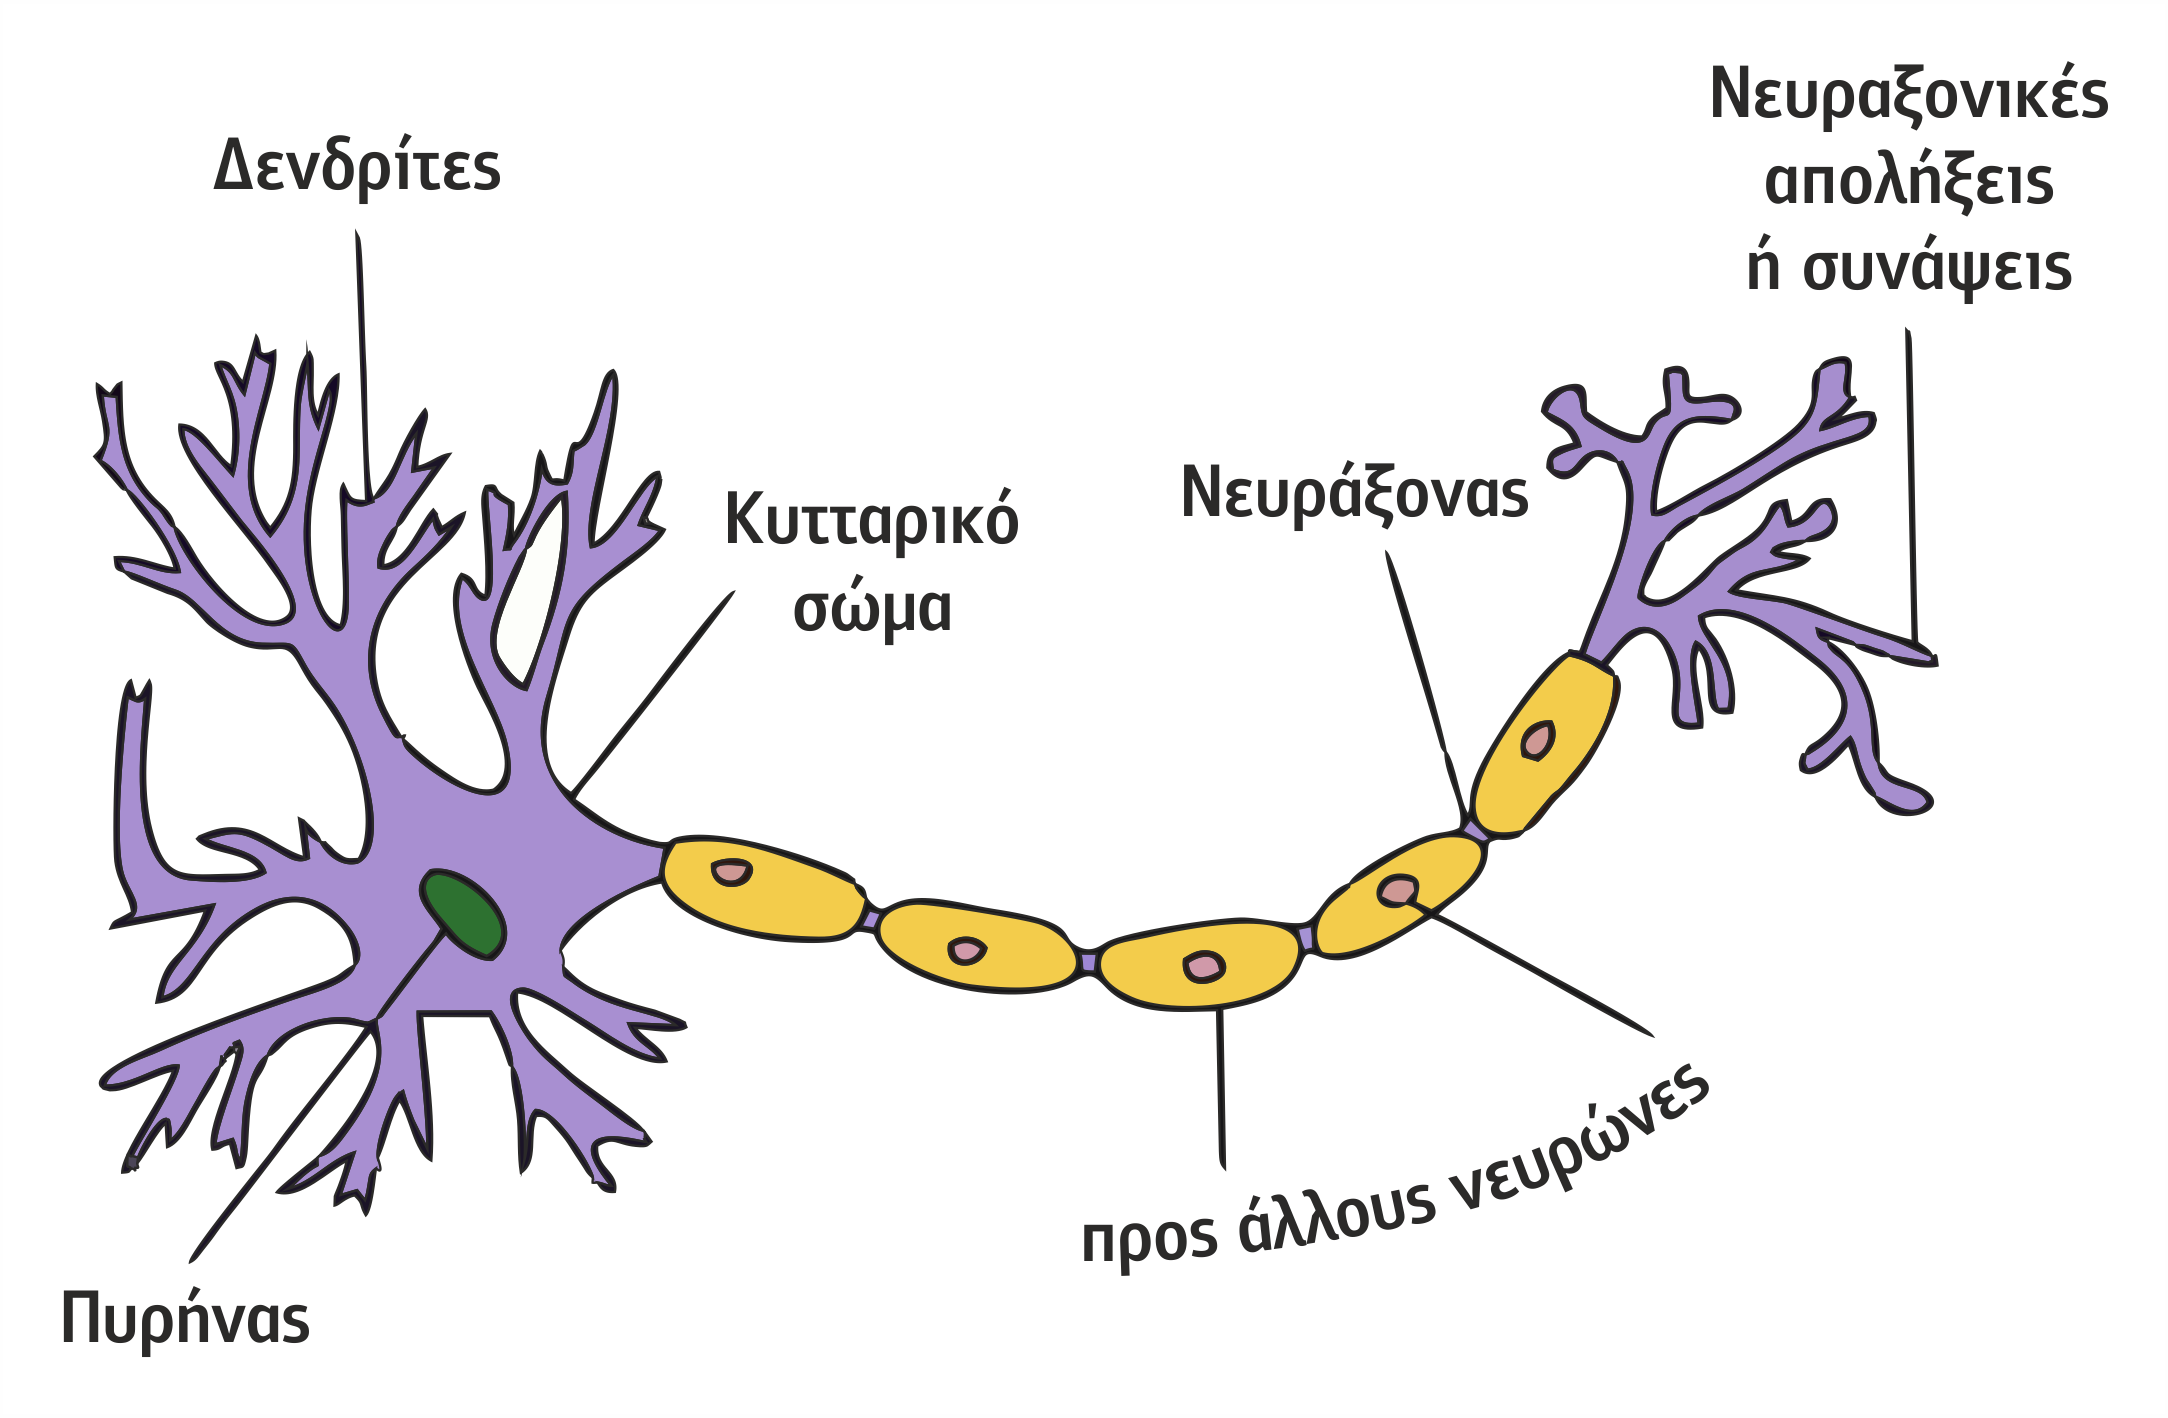
\includegraphics[width=0.7\textwidth]{./images/chapter3/neuron.png}
  \caption[Βιολογικός Νευρώνας]{Βιολογικός νευρώνας.}
  \label{fig:neuron_bio}
\end{figure}
Στο \autoref{fig:neuron_bio} φαίνεται η
μορφή και tα μέλη ενός βιολογικού νευρώνα, ενώ το αντίστοιχο μαθηματικό
μοντέλο παρουσιάζεται στο \autoref{fig:neuron_model}.
Τα κύρια μέρη του βιολογικού νευρώνα είναι τα εξής:
\begin{itemize}
  \item{\textbf{Δενδρίτης (Dendrites)}: Δέχεται είσοδο από άλλους νευρώνες.}
  \item{\textbf{Σώμα του κυττάρου (Cell body)}: Εξάγει συμπεράσματα, με βάση τις εισόδους.}
  \item{\textbf{Νευράξονες (Axon terminals)}: Συνδέει την έξοδο που λαμβάνεται από το σώμα του κυττάρου με την
    είσοδο άλλων νευρώνων.}
\end{itemize}

\begin{figure}[!ht]
  \centering
  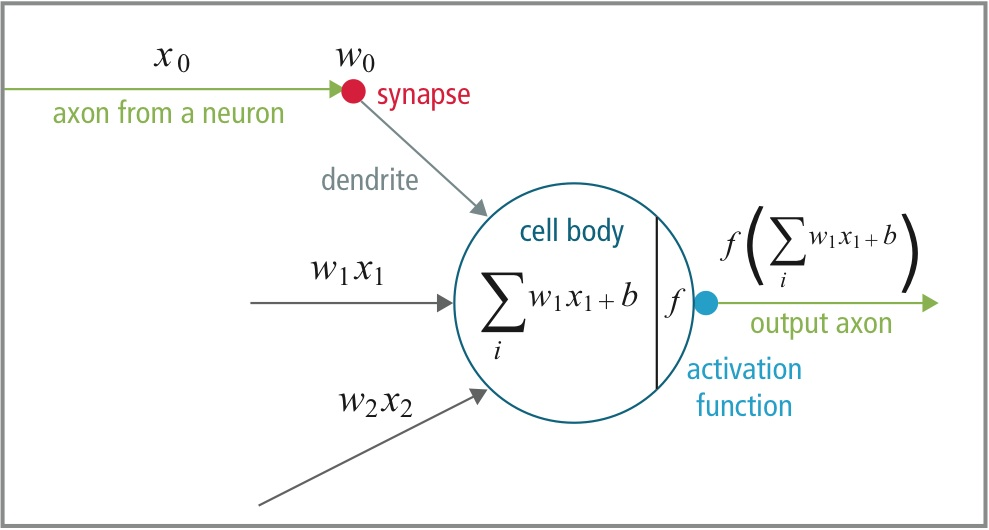
\includegraphics[width=0.8\textwidth]{./images/chapter3/neuron_model.jpg}
  \caption[Μαθηματικό μοντέλο του νευρώνα]{Μαθηματικό μοντέλο του νευρώνα}
  \label{fig:neuron_model}
\end{figure}

Continue...
% The area of Neural Networks has originally been primarily inspired by the goal of modeling biological neural systems, but has since diverged and become a matter of engineering and achieving good results in Machine Learning tasks. Nonetheless, we begin our discussion with a very brief and high-level description of the biological system that a large portion of this area has been inspired by.
% Resource: http://cs231n.github.io/neural-networks-1/

\subsection{Multilayer Perceptron - MLP}

TODO!

\subsection{Συναρτήσεις Ενεργοποίησης}

TODO!

\subsection{Ο αλγόριθμος Backpropagation}

TODO!

\subsection{Αρχιτεκτονικές}

TODO!
